\section{Optimization system}
\label{sec:os_implementation}

Given a FTP request, the Optimization System (OS) is the module that constructs the respective solutions, using the strategies described in subsection \ref{sec:os_design}. This module is constructed using the Python3 programming language, and uses the \textit{numpy} library \cite{numpy} for the construction and the management of the multi-dimensional (and often large) arrays, which describe an FTP instance.   

The developed optimization system implements each of the three proposed optimization strategies: the nearest neighbour heuristic, the ACO and the SA metaheuristics (section \ref{sec:sa}). Given the straightforward implementation of the nearest neighbour, its implementation will not be discussed. Instead, this subsection will focus on the implementation details of the ACO and the SA metaheuristics.

The implementation of the ACO follows the methodology described in subsection \ref{sec:aco} and is illustrated in figure \ref{fig:aco_flow}. This metaheuristic receives, as input, a structure describing the FTP requests, which includes the weight matrix  and the constraints of the problem. This metaheuristic starts by initializing the algorithmic specific parameters, using the values defined in table \ref{tab:parameters}. It also required the initialization of the pheromone matrix, using equation \ref{eq:tau_zero}. 

\begin{figure}[h]
  \centering
  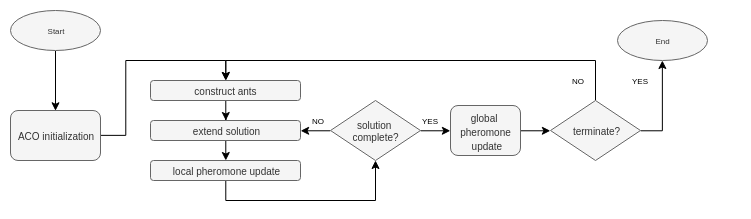
\includegraphics[width=\textwidth]{./Figures/system_implementation/aco_flow.png}
  \caption{Flowchart of the implemented Ant Colony System procedure.}
  \label{fig:aco_flow}  
\end{figure}

This is followed by the initialization of all ants belonging to the colony. Each ant is implemented as an independent thread, which allows for the colony to run in a parallel way. Thus, all ants construct a solution to the problem in an autonomous way, using the transition rules described in equations (\ref{eq:selection_rule}, \ref{eq:exploitation}, \ref{eq:exploration}). At each step of the solution construction process, it is necessary to apply a local pheromone update, by applying \ref{eq:local_update}, which decreases the probability of that solution component being selected by other ants, in the same iteration. After each ant finishes the construction of a solution, it is necessary perform the pheromone update (equation \ref{eq:pheromone_update}), as to reflect the search experience. Given that each ant is an independent thread, it is necessary to lock the pheromone matrix as to protect it from being accessed by multiple threads at the same time.

In its turn, the implementation of the SA follows the methodology described in subsection \ref{sec:sa}, as is illustrated in figure \ref{fig:sa_flow}. As happens with the ACO, the SA metaheuristics receives as input the relevant data to describe the FTP, and initializes its algorithmic specific parameters according to table \ref{tab:parameters}. This is followed by the construction of the cooling schedule. To do so, it is necessary to construct a number of solutions, as to calculate the average difference in the objective function, which allows the calculation of the initial temperature (equation \ref{eq:t_zero}) and cooling parameter (equation \ref{eq:lambda}). 

\begin{figure}[h]
  \centering
  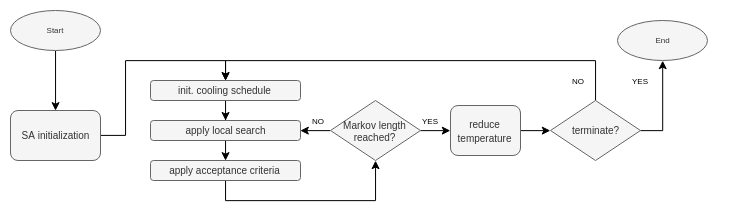
\includegraphics[width=\textwidth]{./Figures/system_implementation/sa_flow.png}
  \caption{Flowchart of the implemented Simulated Annealing procedure.}
  \label{fig:sa_flow}  
\end{figure}

After this initialization process, the SA metaheuristics starts the optimization process by generating a candidate solution, by applying a local search procedure (2-opt) to the current solution. To accept this solution, it is necessary to apply the Metropolis acceptance criteria (equation \ref{eq:metropolis_acceptance}). This process, called Markov cycle, is repeated for a given number of times. Unlike the ACO implementation, the solution construction process of the implemented SA follows a serial approach. After each Markov cycle, the temperature of the system is reduced, by applying equation \ref{eq:cooling}. As the temperature decreases, the algorithm becomes increasingly greedy and converges to a local optimum.

Both metaheuristics have a stop-criteria which is evaluated at the beginning of each solution construction cycle (the ants construction procedure, and the Markov cycle). This criteria is either set to a maximum number of iterations, or to a maximum allowable execution time. When the stop-criteria is reached, these heuristics return the best solution found so far. It is worth noting that this solution corresponds to a set of solution components, arcs, which define both the pair of cities and the schedule of the arc traversal. However, it does not correspond to a set of flights. If the problem under resolution is a real-world flight problem, it is necessary to construct the corresponding set of flight data.


\begin{table}[t]
\centering
\caption{Algorithm specific parameters.}
\label{tab:parameters}
\begin{tabular}{c l c}
\hline
Alg.    &           Parameter         &       Value \\ \hline
%\multirow{2}{*}{FTP}    &           Cost weight ($w_p$)               &         0.7 \\
%                        &           Duration weight ($w_d$)               &         0.3 \\ \hline 
\multirow{5}{*}{ACO}    &           Pheromone relative influence ($\alpha$)              &         1 \\
                        &           Heuristic relative influence ($\beta$)               &         5 \\
                        &           Pheromone evaporation rate ($\rho$)                  &       0.1 \\
                        &           Exploration rate ($Q_0$)                  &       0.9 \\ 
                        &           Number of ants ($m$)                     & 10 \\ \hline
\multirow{6}{*}{SA}     &           First iter. acceptance prob. ($p_0$)                   & 0.98  \\ 
                        &           Last iter. acceptance prob. ($p_f$)                   & $10^{-300}$  \\
                        &           Initial temperature ($t_0$)                   & see Eq.~\ref{eq:t_zero} \\
                        &           Final temperature ($t_f$)                   & see Eq.~\ref{eq:cooling}  \\
                        &           Cooling parameter ($\lambda$)               & see Eq.~\ref{eq:lambda} \\
                        &           Markov chain length ($M$)                     & $N$ \\ \hline
                         
\end{tabular}
\end{table}

